% mnras_template.tex
%
% LaTeX template for creating an MNRAS paper
%
% v3.0 released 14 May 2015
% (version numbers match those of mnras.cls)
%
% Copyright (C) Royal Astronomical Society 2015
% Authors:
% Keith T. Smith (Royal Astronomical Society)

% Change log
%
% v3.0 May 2015
%    Renamed to match the new package name
%    Version number matches mnras.cls
%    A few minor tweaks to wording
% v1.0 September 2013
%    Beta testing only - never publicly released
%    First version: a simple (ish) template for creating an MNRAS paper

%%%%%%%%%%%%%%%%%%%%%%%%%%%%%%%%%%%%%%%%%%%%%%%%%%
% Basic setup. Most papers should leave these options alone.
\documentclass[a4paper,fleqn,usenatbib]{mnras}

% MNRAS is set in Times font. If you don't have this installed (most LaTeX
% installations will be fine) or prefer the old Computer Modern fonts, comment
% out the following line
\usepackage{newtxtext,newtxmath}
% Depending on your LaTeX fonts installation, you might get better results with one of these:
%\usepackage{mathptmx}
%\usepackage{txfonts}

% Use vector fonts, so it zooms properly in on-screen viewing software
% Don't change these lines unless you know what you are doing
\usepackage[T1]{fontenc}
\usepackage{ae,aecompl}

\usepackage{mhchem}



\usepackage{graphicx}
\usepackage{subcaption}
\usepackage{float}

\usepackage{color}
\usepackage{booktabs,chemformula}
\usepackage[export]{adjustbox}

\usepackage{verbatim}
\usepackage{tabularx}

\usepackage{caption}
\usepackage{subcaption}
\usepackage{amsmath}

\usepackage{tikz}
\usepackage{hyperref}
\usepackage{longtable}
\usepackage{color}
\newcommand{\todo}[1]{\textcolor{red}{#1}}


\newcommand{\LamostGiants}{454180}
\newcommand{\project}[1]{\emph{#1}}
\newcommand{\lamost}{\project{LAMOST}}
\newcommand{\apogee}{\project{APOGEE}}

\newcommand{\tc}{\project{The Cannon}}

\newcommand{\teff}{T_{\rm eff}}
\newcommand{\logg}{\log_{10}[g\,({\rm cm\,s}^{-2})]}

%%%%%%%%%%%%%%%%%%% TITLE PAGE %%%%%%%%%%%%%%%%%%%

% Title of the paper, and the short title which is used in the headers.
% Keep the title short and informative.
\title[Short title, max. 45 characters]{Mg Depleted and K Enriched Stars from LAMOST Spectral Data}

% The list of authors, and the short list which is used in the headers.
% If you need two or more lines of authors, add an extra line using \newauthor
\author[Kemp et al.]{
Alex J. Kemp,$^{1}$\thanks{E-mail: ajkem1@student.monash.edu}
Andrew R. Casey,$^{1,2}$
%Matthew Miles? (Monash)
%Brodie Norfolk? (Monash)
%Amanda Karakas? (Monash)
%John Lattanzio? (Monash)
%Kevin Schlaufman? (JHU)
%Anna Ho? (Caltech)
\\
% List of institutions
$^{1}$School of Physics \& Astronomy, Monash University, Clayton 3800, Victoria, Australia\\
$^{2}$ Faculty of Information Technology, Monash University, Clayton 3800, Victoria, Australia\\
}

% These dates will be filled out by the publisher
\date{Accepted 2018 XX XX. Received 2018 YY YY; in original form 2018 ZZ ZZ}

% Enter the current year, for the copyright statements etc.
\pubyear{2018}


\begin{document}
\label{firstpage}
\pagerange{\pageref{firstpage}--\pageref{lastpage}}
\maketitle

% Abstract of the paper
\begin{abstract}

Stellar absorption spectra act as a record of the primordial conditions within which the star formed. Stars displaying unusual elemental abundances provide are of particular interest; these rare stars often offer clues about astrophysical events and objects that may no longer exist in our galaxy. Stars with  depleted Mg and enhanced K abundances, measured as [Mg/Fe] and [K/Fe], have thus far only been found in the two massive globular clustersr NGC 2419 and NGC 2808. The origin of this abundance signature remains unknown, as does the reason for its apparent exclusivity to these two globular clusters. A satisfactory explanation for this signature has potential to influence theories of globular cluster formation and shed light on the long-standing problem of the underestimation of stars with typical galactic values of [K/Fe]. The apparent exclusivity of this Mg-K anti-correlation to globular clusters is the focus of this survey. Here we present 113 candidate field stars (from a sample size of \LamostGiants \ giants from \lamost \ DR2) that have spectra consistent with anomalously depleted [Mg/Fe] and enhanced [K/Fe] abundances, though none with abundances comparable to the extreme population of stars identified in NGC 2419.


%454180 RGB stars from the low resolution LAMOST DR2 survey were searched for anomalously high K and depleted Mg signatures. This study represents the largest search for field stars containing the Mg-K anti-correlation so far identified only in the globular NGC 2419 and NGC 2808. 23 stars displaying absorption spectra with over-abundant K and depleted Mg accross a range of metalicities were identified, but none were identified as having [Mg/Fe] or [K/Fe] consistent with the Mg depleted population found in NGC 2419. The abundances in these 23 stars are estimated at ranging between [INSERT RANGE FOR K AND MG HERE BASED OFF LAMOST DATA]. High resolution spectra for three stars (1 of which is not included among the final count of 23 spectral candidates for the signiature for reasons relating to the LAMOST signal quality for that star, despite having the highest K abundance of the three at [K/Fe]=1.54) selected based on observability characteristics were obtained using the Las Campanas Observatory, and for these stars elemental abundances for heavy elements such as Sc and V are also presented.
\end{abstract}

% Select between one and six entries from the list of approved keywords.
% Don't make up new ones.
\begin{keywords}
keyword1 -- keyword2 -- keyword3
\end{keywords}

%%%%%%%%%%%%%%%%%%%%%%%%%%%%%%%%%%%%%%%%%%%%%%%%%%

%%%%%%%%%%%%%%%%% BODY OF PAPER %%%%%%%%%%%%%%%%%%

\section{Introduction}

NGC 2419 is the Milky Way's third most massive globular cluster, and its chemical composition makes it perhaps the most unusual star cluster in the Galaxy. Recent spectroscopic studies of red giant branch (RGB) stars in NGC 2419 revealed a strong anti-correlation between Mg and K abundances in nearly half of the studied stars, and weaker abundance relations in Si, Sc, Ca, Ti and V \citep{mucciarelli2012,cohenkirby2012}. Depletions of Mg within dwarf spheroidal (dSph) galaxies are not rare \citep{mucciarelli2012}, but are always accompanied with an increase in [Fe/H].
%\todo{[citations needed; possibly remove. RESOLVED, addapted statement slightly. relevant sources: Mucciarreli and Tsujimoto.]}
The mechanism for this Mg depletion is the introduction of $\alpha$-poor and Fe-rich material released from Type Ia supernovae \citep{tsujimoto2012first} which locally pollutes the more `normal' [Mg/Fe] ratios that arise from Type II supernovae. However, the two populations in NGC 2419 are indistinguishable in their [Fe/H] abundance \citep{cohenkirby2012}. Furthermore, Type Ia supernovae enrichment cannot account for the enhanced K abundance or the similar  abundance trends observed in NGC 2419. Currently there is no known nuclear process that can explain the Mg-K abundance variations  without invoking unrealistic temperature conditions or by altering reaction rates by several orders of magnitude. 




%Recently \cite{youngwooklee} used a Ca filter to identify two population in NGC 2419 corresponding to two generations of stars: G1, first generation metal poor stars, and G2, second generation stars displaying enhanced Ca and significantly increased He abundance ($\Delta Y = 0.19$). The Mg depleted population identified previously was found to be contained with the G2 population.

A  targeted search looking [K/Fe] in RGB stars from clusters NGC 6752, NGC 6121, NGC 1904, and $\omega$ Centauri as well as 21 field stars 
%\todo{21 field stars or 21 clusters?? I thought carretta looked at lots of clusters, no?} RESOLVED: Info accurate, no action taken.
 found in all cases K abundances falling within the bounds of the Mg normal population in NGC 2419 \citep{carretta2013}.
 % \todo{The exception is NGC 2808......} RESOLVED: Rephrased paragraph.
NGC 2808 is the only cluster other than NGC 2419 where the anticorrelation between Mg and K has been observed. All 4 of its known Mg depleted stars have been found to have an anti-correlation with K \citep{mucciarelli2015}, although the amplitude of these abundances was weaker than that in NGC 2419. The fact that the Mg-K anti-correlation is apparently confined to these very few globular clusters would seem to imply either a small population  of unusual polluter stars of some sort or a single extremely massive polluter star.

An early modelling attempt at replicating the anomalous Mg/K abundances assumed hot-bottom burning in AGB and super-AGB (SAGB) stars \citep{ventura2012}. This study succeeded in reproducing the Mg-K anti-correlation through the nuclear reaction pathway \ce{^{36}Ar(p,\gamma)^{37}K(\beta ^+ \nu)^{37}Ar(e^-,\nu)^{37}Cl(p,\gamma)^{38}Ar(p,\gamma)^39K} (corrected as per \cite{iliadis2016}) \todo{Ask andy if its right to cite iliadis here, and why he removed the 'corrected as per' bit.} for the production of K. However, abundance patterns consistent with NGC 2419 were only achievable if the reaction cross section was set to 100 times the commonly accepted rate or if the temperature at the base of the envelope  temperatures could be made to exceed $\sim$ 150 K.

A more recent attempt to replicate the Mg/K abundance signature in NGC 2419 by \cite{iliadis2016} also attempted to reproduce the abundances of Si, Sc, Ca, Ti and V  \citep[elements reported as having weak correlations with Mg by][]{cohenkirby2012}. The ultimate goal was to constrain the temperatures and densities required to produce the chemical signature, and thereby provide insight into potential polluter candidates. It is perhaps noteworthy that they identified a different main reaction pathway for K nucleosynthesis to that of \cite{ventura2012}, which is relegated to a minor minor secondary pathway. The main pathway they identify is \ce{^{36}Ar(p,\gamma)^{37}K(\beta ^+ \nu)^{37}Ar(p,\gamma)^{38}K(\beta ^+ \nu)^{38}Ar(p,\gamma)^39K}. 


It was found that (excepting the case of extremely high densities > $10^8$ g/cm$^3$) temperatures between 100 and 200 MK and densities between 10$^{-4}$ and 10$^8$ g/cm$^3$ were required. Using this information, core and shell burning of low mass, high mass and super massive stars were ruled out as potential polluter candidates, as well as regular AGB stars. Super-AGB (SAGB) stars however were regarded as potential candidates, with only a relatively small (roughly 10-20 MK) increase in temperature required to fall in the acceptable band of parameter space identified. The other potential candidate identified was novae, although the lack of detailed models of white dwarf accretion of material similar to that of NGC 2419 either from a binary companion or the intracluster medium limits appraisals of its feasibility regarding whether enough ejecta could be produced and retained by the cluster. However, based on current novae frequency in globular clusters determined by \cite{kato2013novae}, \cite{iliadis2016} conclude that the amount of material that would be produced by Novae is at most 1 \% of the total required mass to pollute 30 \% of NGC 2419.


Another proposed  polluter candidate is a pair-instability super nova (PISN) \citep[PISN;][]{carretta2013}. Unique to extremely massive Population III stars, these events involve the total destruction of the star, with no black hole remnant being left behind. The main argument for this idea is that the extreme rarity of these events, coupled with the huge masses of processed material involved, could potentially allow the entire signature in NGC 2419 to be the result of a single event, explaining why it is not seen in any other globular clusters. However, the signature odd-even proton number abundance pattern associated with PISNs is absent from NGC 2419 \citep{cohenkirby2012}, making this particular scenario unlikely. However, some other type of extremely massive star exploding in a single event would certainly go a long way to explaining the rarity of the signal.
% \todo{Do all the abundance variations like Sc, Si, Ca, Ti, and V go in the expected direction for PISN?} RESOLVED: You are quite correct, I was entirely mistaken. In fact, the odd-even abundance pattern is absent from NGC 2419 in general. segment is edited to reflect this.


%It has been suggested that NGC 2419's position and size, being both very massive and very distant from the Milky Way compared to many other globular clusters, aids it in retaining enriched material from explosive events \citep{mucciarelli2012}. It is also perhaps noteworthy that NGC 2808 is also one of the more massive globular clusters of the Milky Way, although it is far closer to the Galactic Centre. But if this unknown pollution event is common among globular clusters and the cause of its apparent exclusivity to NGC 2808 and NGC 2419 is enhanced ejecta retention due to high mass, then other massive clusters such as $\omega$ Centauri would also be expected contain the signature, which to date has not been observed.

%While it is plausible that the increased mass and greater distance from the gaseous disk of the Milky Way would cause a clusters first generation polluter stars to have an increased effect on the second generation of stars, this effect would apply to all ejecta (assuming comparable energies). So while it might be expected that second generation stars in clusters similar to NGC 2419 made up of more material processed by the first generation than other lighter globular clusters, it doesn't explain why the ejecta from the first generation was apparently dominated by this as yet unknown polluter object resulting in the Mg-K anti-correlation. In the opinion of the author, it is the identity and physical characterisation of this unknown polluter that is of the greatest scientific interest, with such a result also hopefully answering the question of the signatures uniqueness.

Beyond the intrinsic scientific value of identifying the responsible mechanism for the puzzling Mg-K anti-correlation, a satisfactory explanation for this signature could offer insight into the underestimation of K abundances in the Milky Way predicted by models \citep{kobayashi2011}. Such an explanation could also be beneficial to efforts to understand globular cluster formation and evolution.

Here we use \lamost\ data to conduct the largest ever search for field stars that are enhanced in potassium and depleted in magnesium. The discovery (or non-discovery) of such stars will guide models that attempt to explain the Mg-K anti-correlation and related abundance phenomena. \todo{In Section \ref{sec:methods} we outline our methods to identify candidates enhanced in K and depleted in Mg, and the follow-up observations and analysis of those candidates. In Section \ref{sec:discussion} we discuss things. Section \ref{sec:conclusions} contains conclusions.}


%This study, which queries \LamostGiants\ \lamost\ giants for depleted Mg and enhanced K, seeks to provide additional information which can be used to guide and test models attempting to explain the Mg-K anti-correlation and related phenomena. The large sample size provides greater insight into the supposed exclusivity of the signature, and the stars identified present an important opportunity for follow up observations.


\section{Methods, Observations, Simulations etc.}

The data set of \LamostGiants\ \lamost\ giants was prepared by \citet{ho2017} for use with the supervised machine learning code \tc. The \lamost\ data was shifted to rest frame and pseudo-continuum-normalised before it was resampled to a common uniform wavelength grid between 3905\,\AA\ and 9000\,\AA. \tc\ was used to infer $\teff$, $\logg$, [Fe/H], and [$\alpha$/Fe] using 9,952 stars in common between \lamost\ and the higher spectral resolution \apogee\ survey through the use of a data-driven spectral model. For details regarding the preparatory work, model generation, and label transfer between the \apogee\ and \lamost\ surveys, the reader is directed to \citet{ho2017}. 

We identified candidate Mg/K giant stars by searching for significant deviations in flux residuals. The flux residuals were taken as the normalised \lamost\ flux and the best-fitting data-driven model from \tc\ (where $f_{residual} = f_{data} - f_{model}$). A positive residual implies a higher observed normalised flux than expected by the model (less stellar absorption than predicted by the model), while a negative residual implies a lower observed normalised flux than expected (more stellar absorption than predicted by the model). 

We fitted a gaussian profile to the flux residuals for all three absorption lines in the Mg triplet (5167 \AA, 5172 \AA, 5184 \AA) as well as the K doublet (7665 \AA, 7699 \AA) for all \LamostGiants\ giants in \lamost\ data release 2 (DR2). For every star we recorded the profile amplitudes, wavelengths, widths, as well as associated measurement uncertainties of these quantities. We identified candidates by requiring they match at least one of the following three quality filters.
\begin{enumerate}
\item We required the amplitude $A$ of the profile at the Mg 5184 \AA \ line to exceed $A_{{\rm Mg} @ 5184} > 0.05$ and the amplitude of the profile at the K 7665 line to exceed $A_{{\rm K}\,@\,7665} < 0.05$. Both amplitudes must also be measured at more than $3\sigma$ ($|A|/\sigma_{A} \geq 3$).
\item We required two of the three Mg triplet lines to satisfy $A > 0.05$ and at least one K line to have $A < 0.05$, and for those amplitudes to have $|A|/\sigma_{A} \geq 3$.
\item We required two of the three Mg triplet lines to have $A > 0$ and both K lines to have $A < 0$, and for the spectra to have a signal-to-noise ($S/N$) ratio of $S/N > 30$ in \lamost, and a reported $\chi_{r}^2 < 3$ from \tc.
\end{enumerate} 
 
These filters identified 384 unique stars to be vetted manually. We visually inspected every candidate (multiple times) and excluded any candidate that showed any evidence of being a false positive, including candidates that exhibited data reduction issues, apparent absorption that was narrower than the expected spectral resolution, as well as 75 stars that exhibited chromospheric emission at H$\alpha$. The distilled catalogue includes \todo{113} candidate stars enhanced in K and depleted in Mg.


\subsection{Figures and tables}

Figures and tables should be placed at logical positions in the text. Don't
worry about the exact layout, which will be handled by the publishers.

Figures are referred to as e.g. Fig.~\ref{fig:example_figure}, and tables as
e.g. Table~\ref{tab:example_table}.




\begin{figure}
	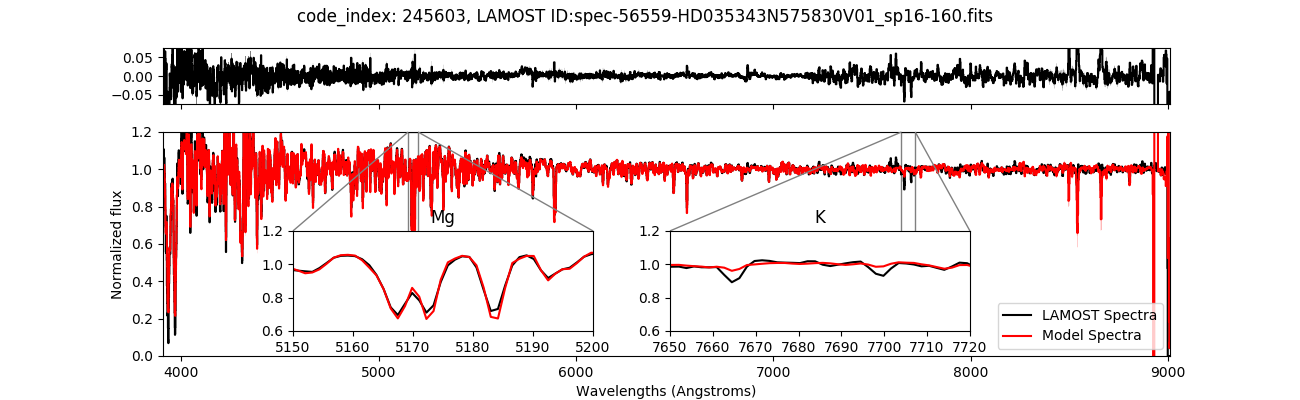
\includegraphics[width=\columnwidth]{posterchildof13.png}
    \caption{Poster Child}
    \label{posterchild}
\end{figure}

\begin{figure}
	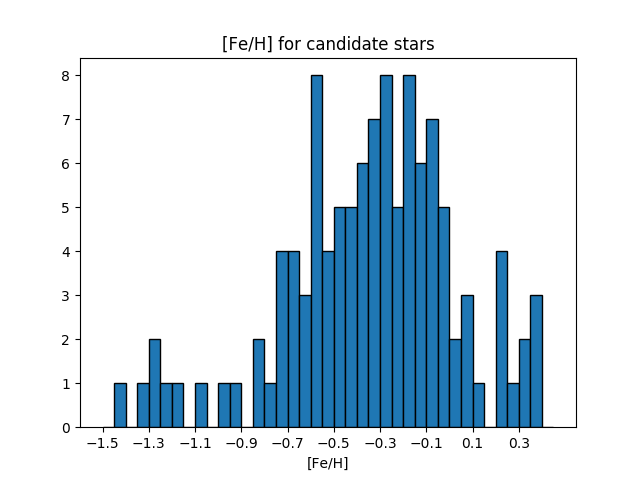
\includegraphics[width=\columnwidth]{histof113.png}
    \caption{Metalicity Histogram}
    \label{mhist}
\end{figure}


\begin{figure}
	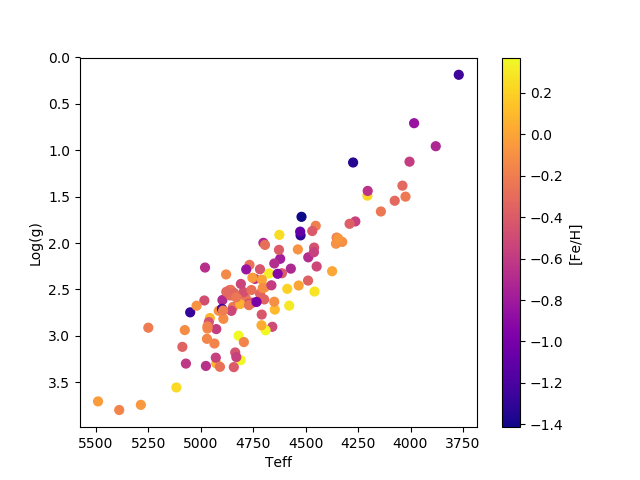
\includegraphics[width=\columnwidth]{loggteffof113.png}
    \caption{Effective temperature, log surface gravity, metalicity}
    \label{tefflogg}
\end{figure}

\begin{figure}
	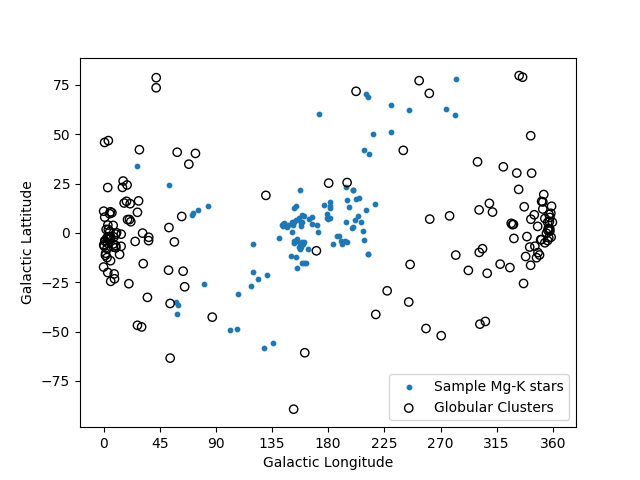
\includegraphics[width=\columnwidth]{globclustof113.png}
    \caption{Galactic coordinates for Mg-K stars and known globular clusters}
    \label{galcord}
\end{figure}

\begin{figure}
	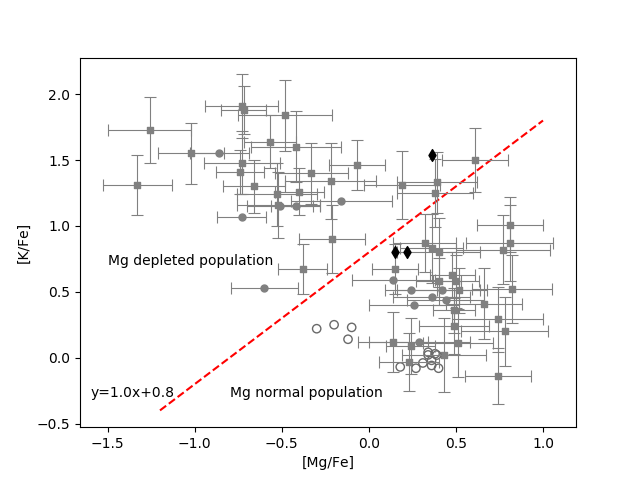
\includegraphics[width=\columnwidth]{KvsMgab.png}
    \caption{[Comparison of K vs Mg abundances with NGC 2419 and NGC 2808.}
    \label{KvsMg}
\end{figure}


% Example table
\begin{table}
	\centering
	\caption{This is an example table. Captions appear above each table.
	Remember to define the quantities, symbols and units used.}
	\label{tab:example_table}
	\begin{tabular}{lccr} % four columns, alignment for each
		\hline
		A & B & C & D\\
		\hline
		1 & 2 & 3 & 4\\
		2 & 4 & 6 & 8\\
		3 & 5 & 7 & 9\\
		\hline
	\end{tabular}
\end{table}

\section{Discussion}

\begin{itemize}
\item Association with globular clusters: basically all stars (will have to redo plot and search for the new tables) are not associated with globular clusters. in terms of those which are kinda close in GC, state which cluster(s) they could be associated with. We lack dynamics information, but potentially the next data release from GAIA will help with that. Check with apparent magnitudes to see if the stars are consistent in that regard.

\item Metalicity: the candidate stars are found at a wide range of metalicities, from \todo{-1.4<[Fe/H]<0.3}. for comparison, NGC 2808 and NGC 2419 have [Fe/H] ~-2.

\item Abundances: K abundances are lower and Mg abundances are higher than those in the extreme population of 2419. however, they \textit{are} still (perhaps) significantly K enhanced and Mg depleted, perhaps the first field stars identified as such. Only 113 out of \LamostGiants \ stars were found to be good candidates for enhanced K and reduced Mg. Likely not products of the same process as acted in NGC 2419, but possibly? Main implications: searched \LamostGiants \ stars, but didn't find any that we could say 'yeah that looks like it could have came from the same process that caused NGC 2419's signiature'.

\item What does this abundance imply about pollution mechanisms? depends whether we decide that our identified stars were produced by the same process or not. IF they weren't produced by the same process, then this is further evidence that the event/object was unique to old globular clusters. If however they WERE produced by the same process, but just weren't as polluted (the primordial material was made up of a lower fraction of anomalously enriched material), then the implications are a bit weird. We found stars across a large range of metalicities. Diferent formation times is also implied by metalicity.



\item spread in Logg and Teff: the fact that we see stars across a range of Teff and Logg eliminates the idea that the candidates as all being so called 'red-clump' red giants or any other phenomena specific to certain RGB stages/ types. 

\item working hypothesis (John, Tout): We decouple the Mg and the K. A SAGB binary with a smaller companion. the SAGB produces K, which then accretes to the companion. the companion will evolve long after the SAGB explodes, then will either (depending on mass/temperature) undergo hot bottom burning or it won't. If it does? undergo hot bottom burning then Na will be produced. If it doesn't? undergo hot bottom burning then Na won't be produced. other predictions: O shouldn't? be be there, nor should C or N as they get turned into Na. This scenario is plausible to happen in the MW disk, throughout an extended period of time, therefore being consistent with the spread in metalicities that we see. Look at iliadis 2017 to see some other implications of hot bottom burning in AGB (low temperature) star and SAGB (high temp) burning.

\item We're not allowed to have a single big event in NGC 2419 and then clumps of material floating round the galaxy and occasionally forming a star. one good reason: its really distant form the galaxy. thus our K enhancements must source from a star inside the galaxy, NOT a globular cluster. this raises some interesting issues. If the source of our K enhancements is the same as NGC 2419, where we had Mg depletions that then were later covered up/ reduced in magnitude in the case of our disk stars, then the big question i'd want answered is: So we have this thing that only occurs in 2419... and the MW disk... throughout the life of the MW disk... but not in any other globular clusters. seems a bit picky...

\item novae: the mass budged problem is much worse for NGC 2419 than \cite{iliadis2016} made it appear, and is very unlikely to be responsible for the phenomena. finding even more K enhanced stars in the MW doesn't change this.


\end{itemize}

\section{Conclusions}

The last numbered section should briefly summarise what has been done, and describe
the final conclusions which the authors draw from their work.

\section*{Acknowledgements}

- LAMOST
- ARC DP (Casey)
- Magellan/MIKE and Australian government
- others???

%%%%%%%%%%%%%%%%%%%%%%%%%%%%%%%%%%%%%%%%%%%%%%%%%%

%%%%%%%%%%%%%%%%%%%% REFERENCES %%%%%%%%%%%%%%%%%%

% The best way to enter references is to use BibTeX:

\bibliographystyle{mnras}
\bibliography{mgkbib} % if your bibtex file is called example.bib


% Alternatively you could enter them by hand, like this:
% This method is tedious and prone to error if you have lots of references


%%%%%%%%%%%%%%%%%%%%%%%%%%%%%%%%%%%%%%%%%%%%%%%%%%

%%%%%%%%%%%%%%%%% APPENDICES %%%%%%%%%%%%%%%%%%%%%

\appendix

\section{Some extra material}
\begin{table}
\centering
\begin{tabular}{llllllllll}
\hline
\textbf{2MASSID} & \textbf{RA} & \textbf{DEC} & \textbf{S/N} & \textbf{Vr (km/s)} & \textbf{Teff} & \textbf{Logg} & \textbf{[Fe/H]} & \textbf{[Alpha/Fe]} & {$\boldsymbol \chi^\textbf{2}$} \\ \hline
J060142.80+132321.4 & 90.43 & 13.39 & 45 & 33.28 & 4858 & 2.57 & -0.30 & 0.10 & 0.24 \\ \hline
J075043.12+204658.0 & 117.68 & 20.78 & 47 & 52.46 & 4795 & 2.53 & -0.47 & 0.06 & 0.40 \\ \hline
J032450.35+352401.8 & 51.21 & 35.40 & 143 & 95.63 & 4908 & 3.33 & -0.27 & 0.19 & 0.70 \\ \hline
J214721.25+023958.7 & 326.84 & 2.67 & 104 & -63.83 & 4649 & 2.22 & -0.68 & 0.26 & 0.81 \\ \hline
J040340.38+563902.4 & 60.92 & 56.65 & 30 & 39.87 & 4459 & 2.05 & -0.46 & 0.01 & 0.61 \\ \hline
J035455.85+594730.3 & 58.73 & 59.79 & 57 & -40.17 & 4956 & 2.81 & 0.08 & 0.04 & 0.56 \\ \hline
J035928.29+595932.8 & 59.87 & 59.99 & 35 & -38.07 & 4808 & 2.44 & -0.53 & 0.16 & 0.32 \\ \hline
J034458.82+592955.1 & 56.25 & 59.50 & 53 & -32.68 & 4811 & 2.66 & 0.06 & 0.10 & 0.64 \\ \hline
J220657.78+232138.3 & 331.74 & 23.36 & 50 & -27.58 & 4842 & 3.34 & -0.40 & 0.10 & 0.23 \\ \hline
J061323.14+325543.0 & 93.35 & 32.93 & 39 & -25.78 & 4861 & 2.51 & -0.40 & 0.16 & 0.42 \\ \hline
J005649.98+391722.9 & 14.21 & 39.29 & 41 & -46.77 & 4578 & 2.67 & 0.31 & 0.10 & 0.44 \\ \hline
J002619.36+565612.1 & 6.58 & 56.94 & 31 & -39.57 & 4205 & 1.49 & 0.22 & 0.06 & 0.76 \\ \hline
J040817.31+463252.5 & 62.07 & 46.55 & 92 & -1.80 & 5019 & 2.68 & -0.09 & 0.05 & 0.98 \\ \hline
J072156.18+225405.3 & 110.48 & 22.90 & 101 & -46.77 & 4840 & 2.54 & -0.33 & 0.17 & 0.69 \\ \hline
J040634.97+411354.9 & 61.65 & 41.23 & 45 & -35.38 & 4770 & 2.67 & -0.26 & 0.07 & 0.51 \\ \hline
J041608.62+433504.7 & 64.04 & 43.58 & 30 & -20.09 & 4967 & 2.90 & -0.17 & 0.04 & 0.33 \\ \hline
J013039.08+404843.8 & 22.66 & 40.81 & 71 & -80.34 & 4355 & 2.01 & -0.09 & 0.14 & 0.93 \\ \hline
J052924.25+494319.7 & 82.35 & 49.72 & 94 & -22.48 & 5087 & 3.12 & -0.35 & 0.11 & 0.70 \\ \hline
J061427.58+331544.3 & 93.61 & 33.26 & 51 & 3.30 & 4468 & 1.87 & -0.41 & 0.11 & 0.67 \\ \hline
J062128.63+343545.8 & 95.37 & 34.60 & 39 & 33.28 & 4831 & 2.58 & -0.23 & 0.08 & 0.27 \\ \hline
J030101.42+560042.3 & 45.26 & 56.01 & 88 & -39.27 & 4878 & 2.53 & -0.32 & 0.09 & 0.67 \\ \hline
J120032.60+024438.2 & 180.14 & 2.74 & 97 & 166.98 & 4633 & 2.33 & -0.93 & 0.26 & 0.89 \\ \hline
J163910.01+100545.3 & 249.79 & 10.10 & 39 & 123.81 & 4663 & 2.46 & -0.58 & 0.03 & 0.61 \\ \hline
\end{tabular}
\caption{My caption}
\label{my-label}
\end{table}

\newpage
\begin{comment}
\begin{table}[H]
\centering
\begin{tabular}{llllllllll}
\hline
\textbf{2MASSID} & \textbf{RA} & \textbf{DEC} & \textbf{S/N} & \textbf{Radial\_Velocity\_(km/s)} & \textbf{Teff} & \textbf{Logg} & \textbf{{[}Fe/H{]}} & \textbf{{[}Alpha/Fe{]}} & \textbf{$\chi^2$} \\ \hline
J234942.32+300654.0 & 357.43 & 30.11 & 20 & -195.46 & 4004 & 1.12 & -0.58 & 0.23 & 2.73 \\ \hline
J065334.23+131639.7 & 103.39 & 13.28 & 7 & 179.88 & 4896 & 2.61 & -0.71 & 0.02 & 0.18 \\ \hline
J112309.75+261255.9 & 170.79 & 26.22 & 3 & 113.02 & 4273 & 1.13 & -1.35 & 0.17 & 0.09 \\ \hline
J111651.71+253038.5 & 169.22 & 25.51 & 6 & 102.83 & 4658 & 2.90 & -0.50 & 0.02 & 0.08 \\ \hline
J045424.86+534628.5 & 73.60 & 53.77 & 6 & -36.57 & 4451 & 1.81 & -0.19 & 0.07 & 0.37 \\ \hline
J065857.80+081714.8 & 104.74 & 8.29 & 12 & 26.68 & 5070 & 3.30 & -0.61 & 0.10 & 0.18 \\ \hline
J045544.93+490023.3 & 73.94 & 49.01 & 6 & -38.07 & 4717 & 2.55 & -0.34 & 0.11 & 0.11 \\ \hline
J040739.62+423724.4 & 61.92 & 42.62 & 9 & -37.77 & 4075 & 1.54 & -0.32 & 0.08 & 0.28 \\ \hline
J043121.48+414757.2 & 67.84 & 41.80 & 8 & -12.59 & 4537 & 2.07 & -0.09 & 0.03 & 0.13 \\ \hline
J041900.21+422223.9 & 64.75 & 42.37 & 12 & -34.18 & 4263 & 1.77 & -0.55 & 0.09 & 0.28 \\ \hline
J041209.44+411801.0 & 63.04 & 41.30 & 35 & -20.69 & 4767 & 2.24 & -0.26 & 0.12 & 0.91 \\ \hline
J063648.82+130723.3 & 99.20 & 13.12 & 8 & 85.74 & 4925 & 2.93 & -0.57 & -0.03 & 0.19 \\ \hline
J070524.04+120351.0 & 106.35 & 12.06 & 19 & 60.26 & 4754 & 2.64 & -0.56 & -0.02 & 0.24 \\ \hline
J063501.25+134744.6 & 98.76 & 13.80 & 7 & 47.67 & 4612 & 2.33 & -0.40 & 0.01 & 0.19 \\ \hline
J053942.83+383727.8 & 84.93 & 38.62 & 18 & -85.74 & 4979 & 2.26 & -0.66 & 0.23 & 0.27 \\ \hline
J053123.26+421952.0 & 82.85 & 42.33 & 8 & 41.07 & 4785 & 2.59 & -0.26 & 0.01 & 0.26 \\ \hline
J052643.65+354130.3 & 81.68 & 35.69 & 9 & -18.89 & 4914 & 2.73 & -0.09 & 0.03 & 0.28 \\ \hline
J064618.82+050545.8 & 101.58 & 5.10 & 9 & 85.74 & 4772 & 2.66 & -0.49 & -0.01 & 0.28 \\ \hline
J063719.82+185602.6 & 99.33 & 18.93 & 5 & 15.29 & 5075 & 2.94 & -0.12 & 0.03 & 0.10 \\ \hline
J072912.52+073436.9 & 112.30 & 7.58 & 9 & 117.52 & 4835 & 3.18 & -0.44 & 0.33 & 0.34 \\ \hline
J193217.91+374505.6 & 293.07 & 37.75 & 28 & -70.15 & 4982 & 2.62 & -0.48 & 0.33 & 0.55 \\ \hline
J192937.24+390211.0 & 292.41 & 39.04 & 6 & -52.16 & 4819 & 3.00 & 0.37 & 0.12 & 0.21 \\ \hline
J010305.95+043445.9 & 15.77 & 4.58 & 90 & 20.69 & 4646 & 2.72 & 0.10 & 0.05 & 1.17 \\ \hline
J235454.61+110356.9 & 358.73 & 11.07 & 12 & -109.72 & 4794 & 3.07 & -0.16 & 0.30 & 0.21 \\ \hline
J000908.89+124821.9 & 2.29 & 12.81 & 10 & -78.55 & 4892 & 2.82 & -0.12 & 0.33 & 0.19 \\ \hline
J220115.66-001432.2 & 330.32 & -0.24 & 47 & 38.37 & 4925 & 3.30 & 0.06 & 0.23 & 0.32 \\ \hline
J064430.22+341606.3 & 101.13 & 34.27 & 9 & -40.17 & 4809 & 3.26 & 0.36 & 0.19 & 0.31 \\ \hline
J002907.61+354701.0 & 7.28 & 35.78 & 15 & -82.74 & 5116 & 3.56 & 0.24 & 0.17 & 0.18 \\ \hline
J033714.25+403015.1 & 54.31 & 40.50 & 34 & -119.32 & 4674 & 2.33 & 0.32 & 0.22 & 0.86 \\ \hline
J074807.22+261514.2 & 117.03 & 26.25 & 16 & -32.98 & 4846 & 2.69 & -0.23 & 0.05 & 0.16 \\ \hline
J032423.46+425429.6 & 51.10 & 42.91 & 23 & -56.74 & 4649 & 2.63 & -0.11 & -0.01 & 0.34 \\ \hline
J055043.44+162021.2 & 87.68 & 16.34 & 24 & 83.64 & 4587 & 2.49 & 0.21 & 0.07 & 0.28 \\ \hline
J055227.43+181628.0 & 88.11 & 18.27 & 28 & 8.09 & 5388 & 3.80 & -0.17 & 0.05 & 0.43 \\ \hline
J055935.08+150252.1 & 89.90 & 15.05 & 23 & 90.84 & 4487 & 2.15 & -0.68 & 0.01 & 4.35 \\ \hline
J063113.14+015900.3 & 97.80 & 1.98 & 14 & 78.55 & 4879 & 2.34 & -0.13 & 0.01 & 0.56 \\ \hline
J111550.58+104203.9 & 168.96 & 10.70 & 9 & 114.82 & 4519 & 1.72 & -1.41 & 0.32 & 0.17 \\ \hline
J111022.65+171251.0 & 167.59 & 17.21 & 12 & 247.33 & 4524 & 1.92 & -1.30 & 0.13 & 0.30 \\ \hline
J100054.32+185535.5 & 150.23 & 18.93 & 17 & 149.00 & 4373 & 2.30 & 0.01 & 0.01 & 0.39 \\ \hline
J055908.72+210037.7 & 89.79 & 21.01 & 6 & 55.76 & 4325 & 1.99 & -0.10 & -0.03 & 0.75 \\ \hline
J055704.30+215000.1 & 89.27 & 21.83 & 9 & 49.77 & 4691 & 2.94 & 0.37 & 0.00 & 0.30 \\ \hline
J104800.91+424311.0 & 162.00 & 42.72 & 6 & 163.99 & 5050 & 2.75 & -1.29 & 0.12 & 0.18 \\ \hline
J075129.58+024136.9 & 117.87 & 2.69 & 18 & 128.61 & 4741 & 2.39 & -0.61 & 0.05 & 0.28 \\ \hline
J064132.46+580400.9 & 100.39 & 58.07 & 24 & -11.69 & 5285 & 3.74 & -0.06 & 0.07 & 0.36 \\ \hline
J063908.57+381728.0 & 99.79 & 38.29 & 5 & 25.78 & 4853 & 2.73 & -0.52 & 0.02 & 0.17 \\ \hline
J102104.26+105617.4 & 155.27 & 10.94 & 17 & 171.48 & 4526 & 1.88 & -1.09 & 0.07 & 0.28 \\ \hline
J061228.04-040304.1 & 93.12 & -4.05 & 16 & -1.50 & 4928 & 3.24 & -0.56 & 0.09 & 0.19 \\ \hline
J061144.17-040845.1 & 92.93 & -4.15 & 23 & 84.54 & 4709 & 2.77 & -0.42 & -0.00 & 0.24 \\ \hline
J074848.57+210655.5 & 117.20 & 21.12 & 9 & 101.33 & 4447 & 2.25 & -0.52 & 0.04 & 0.11 \\ \hline
J092124.00+204559.5 & 140.35 & 20.77 & 12 & 125.31 & 4570 & 2.28 & -0.71 & 0.06 & 0.31 \\ \hline
J074146.65+145330.5 & 115.44 & 14.89 & 6 & 105.53 & 4701 & 2.00 & -0.71 & 0.04 & 0.18 \\ \hline
J073641.12+164710.6 & 114.17 & 16.79 & 6 & 90.84 & 4621 & 2.17 & -0.77 & 0.01 & 0.26 \\ \hline
J175211.80+273546.6 & 268.05 & 27.60 & 7 & -33.58 & 5489 & 3.71 & -0.03 & 0.14 & 0.15 \\ \hline
J194028.76+504047.6 & 295.12 & 50.68 & 22 & -61.76 & 4352 & 1.94 & -0.17 & 0.23 & 0.35 \\ \hline
J213914.06+025536.2 & 324.81 & 2.93 & 29 & 57.78 & 4488 & 2.40 & -0.37 & 0.05 & 0.46 \\ \hline
J011949.36+063411.4 & 19.96 & 6.57 & 479 & -28.18 & 4820 & 2.61 & -0.29 & 0.09 & 2.38 \\ \hline
J041055.45+570542.6 & 62.73 & 57.10 & 16 & -32.38 & 4141 & 1.66 & -0.23 & 0.07 & 0.47 \\ \hline
J035840.66+574934.5 & 59.67 & 57.83 & 17 & -56.06 & 4693 & 2.02 & -0.28 & 0.14 & 0.46 \\ \hline
J034552.01+595739.3 & 56.47 & 59.96 & 17 & -48.57 & 4627 & 2.07 & -0.38 & 0.16 & 0.41 \\ \hline
J193130.64+432204.2 & 292.88 & 43.37 & 16 & -92.64 & 4934 & 3.08 & -0.16 & 0.30 & 0.26 \\ \hline
J042753.62+365550.6 & 66.97 & 36.93 & 8 & -30.08 & 5249 & 2.91 & -0.21 & 0.18 & 0.30 \\ \hline
J061808.85+313338.2 & 94.54 & 31.56 & 12 & 42.57 & 4970 & 3.03 & -0.15 & 0.10 & 0.55 \\ \hline
J050740.59+492955.0 & 76.92 & 49.50 & 15 & 18.29 & 3879 & 0.96 & -0.72 & 0.06 & 0.54 \\ \hline
J050606.74+494925.0 & 76.53 & 49.82 & 25 & -28.78 & 4857 & 2.50 & -0.25 & 0.12 & 0.34 \\ \hline
J050551.93+493726.0 & 76.47 & 49.62 & 15 & -18.59 & 4961 & 2.85 & -0.47 & 0.07 & 0.27 \\ \hline
J051046.05+523848.3 & 77.69 & 52.65 & 47 & -46.17 & 4697 & 2.61 & -0.34 & 0.26 & 1.03 \\ \hline
J041321.95+520135.7 & 63.34 & 52.03 & 19 & -51.35 & 4694 & 2.48 & -0.05 & 0.05 & 0.50 \\ \hline
J065356.76+344513.1 & 103.49 & 34.75 & 21 & -23.38 & 4533 & 2.46 & -0.00 & 0.15 & 0.28 \\ \hline
J003451.10+424543.0 & 8.71 & 42.76 & 15 & -79.15 & 4460 & 2.10 & -0.56 & 0.24 & 0.31 \\ \hline
J040034.51+472103.8 & 60.14 & 47.35 & 18 & -55.82 & 4708 & 2.39 & -0.01 & 0.10 & 0.65 \\ \hline
J041304.73+470013.8 & 63.27 & 47.00 & 17 & 19.19 & 4290 & 1.79 & -0.37 & 0.03 & 0.79 \\ \hline
J035633.86+463749.2 & 59.14 & 46.63 & 17 & -54.93 & 4753 & 2.37 & -0.05 & 0.12 & 0.34 \\ \hline
J053627.38+581132.8 & 84.11 & 58.19 & 28 & -32.94 & 4457 & 2.52 & 0.28 & 0.05 & 0.49 \\ \hline
J052516.26+585912.5 & 81.32 & 58.99 & 19 & -75.07 & 4023 & 1.50 & -0.22 & 0.05 & 0.51 \\ \hline
J034826.25+350123.4 & 57.11 & 35.02 & 100 & -47.97 & 4710 & 2.89 & 0.04 & 0.38 & 4.72 \\ \hline
J035652.48+325937.2 & 59.22 & 32.99 & 24 & -20.99 & 4038 & 1.38 & -0.31 & 0.08 & 0.55 \\ \hline
J035345.63+340429.3 & 58.44 & 34.07 & 15 & -34.48 & 4830 & 3.23 & -0.56 & 0.06 & 0.14 \\ \hline
J042245.32+430359.8 & 65.69 & 43.07 & 16 & -35.08 & 4967 & 2.92 & -0.13 & 0.03 & 0.20 \\ \hline
J042241.36+414255.6 & 65.67 & 41.72 & 15 & -92.76 & 4975 & 3.32 & -0.66 & 0.02 & 0.27 \\ \hline
J053148.24+225045.6 & 82.95 & 22.85 & 15 & 11.69 & 3982 & 0.71 & -0.84 & 0.08 & 0.63 \\ \hline
J120844.42-012151.8 & 182.19 & -1.36 & 18 & 143.30 & 4783 & 2.28 & -0.84 & 0.28 & 0.48 \\ \hline
J091825.49+172114.5 & 139.61 & 17.35 & 11 & 232.04 & 4898 & 2.71 & -1.19 & 0.29 & 0.14 \\ \hline
J123413.43+160353.7 & 188.56 & 16.06 & 10 & 316.88 & 4734 & 2.63 & -0.99 & 0.03 & 0.17 \\ \hline
J054656.93+442800.0 & 86.74 & 44.47 & 17 & -41.37 & 4758 & 2.51 & -0.27 & 0.09 & 0.15 \\ \hline
J053423.46+460026.9 & 83.60 & 46.01 & 21 & -40.77 & 4893 & 2.73 & -0.18 & 0.10 & 0.26 \\ \hline
J052814.58+511912.4 & 82.06 & 51.32 & 16 & -64.76 & 4344 & 1.95 & -0.06 & 0.10 & 0.51 \\ \hline
J044403.36+543203.6 & 71.01 & 54.53 & 19 & -71.05 & 4625 & 1.91 & 0.25 & 0.07 & 1.42 \\ \hline
J043503.82+552514.6 & 68.77 & 55.42 & 19 & 9.59 & 4704 & 2.48 & -0.11 & 0.04 & 0.60 \\ \hline
J043418.64+535250.2 & 68.58 & 53.88 & 17 & -141.15 & 4204 & 1.44 & -0.64 & 0.19 & 0.76 \\ \hline
J070937.38+201517.2 & 107.41 & 20.25 & 9 & 148.10 & 3770 & 0.19 & -1.24 & 0.04 & 0.46 \\ \hline
J064032.35+335207.5 & 100.13 & 33.87 & 8 & -34.48 & 4717 & 2.28 & -0.44 & 0.24 & 0.24 \\ \hline
\end{tabular}
\caption{Remaining candidates}
\label{Resttab}
\end{table}
\end{comment}

%%%%%%%%%%%%%%%%%%%%%%%%%%%%%%%%%%%%%%%%%%%%%%%%%%


% Don't change these lines
\bsp	% typesetting comment
\label{lastpage}
\end{document}

% End of mnras_template.tex